\documentclass[11pt]{article}
\usepackage[margin=1in]{geometry}
\usepackage{booktabs}
\usepackage{float}
\usepackage{graphicx}
\usepackage{amsmath}
\usepackage{amssymb}
\usepackage{hyperref}
\usepackage{url}

\title{\textbf{Project 1: Exploratory Data Analysis and Simple Regression}\\\large CSCI 4360 / DATA SCIENCE ML II}
\author{Adithya Lakshmikanth, Amy Vu, Aastha Mishra, Ellie Truong, Disha Dhangar}
\date{\today}

\begin{document}
\maketitle

\begin{abstract}
This report presents an exploratory data analysis (EDA) and simple linear regression study across three benchmark datasets from the UCI Machine Learning Repository: Auto MPG (392 rows, 8 columns), Concrete Compressive Strength (1,030 rows, 9 columns), and Airfoil Self-Noise (1,503 rows, 6 columns). A dual-tool implementation methodology was conducted using ScalaTion (Scala 3) and Statsmodels (Python). Preprocessing decisions regarding string categorical attributes, missing value handling, and Tukey outlier diagnostics are documented. For each dataset, complete descriptive statistics and correlation matrices are analyzed, and univariate regression models are estimated for the top two predictors ranked by target correlation. Numerical parameters and quality-of-fit metrics are verified to match identically across ScalaTion and Statsmodels.
\end{abstract}

\section{Introduction and Data Ingestion Architecture}
In data science pipelines, rigorous exploratory data analysis provides crucial understanding of underlying data distributions, collinearity structures, and potential model limitations prior to complex modeling. 

In ScalaTion, data ingestion can be accomplished via three primary mechanisms depending on file structure and schema complexity:
\begin{enumerate}
    \item \textbf{\texttt{MatrixD.load} (in \texttt{scalation.mathstat}):} Directly loads dense numerical CSV data into a matrix representation (\texttt{MatrixD}). Suitable for purely numeric datasets where headers or metadata columns are skipped.
    \item \textbf{\texttt{MatrixD.loadStr} (in \texttt{scalation.mathstat}):} Ingests text files containing categorical or string columns, automatically mapping discrete textual entries to ordinal integer codes via supplied string dictionaries (\texttt{VectorS}).
    \item \textbf{\texttt{Table.load} (in \texttt{scalation.database.table}):} Ingests CSV files into a relational table abstraction (\texttt{Table}), providing explicit domain typing, attribute projection, schema validation, and conversion to numeric regression matrices via \texttt{.toMatrixV(...)}.
\end{enumerate}

All three benchmark datasets were curated into standardized numeric CSV files in \texttt{project1/data/processed/}, loaded into ScalaTion via \texttt{MatrixD.load}, and simultaneously analyzed in Python using Statsmodels.


\section{Auto MPG Dataset}

\subsection{Data Description and Preprocessing}
The Auto MPG dataset was retrieved from the UCI Machine Learning Repository (\url{http://archive.ics.uci.edu/ml/machine-learning-databases/auto-mpg/auto-mpg.data}). The finalized analysis matrix consists of \textbf{392 observations} and \textbf{8 columns} (including response variable \texttt{mpg}).

\begin{itemize}
    \item \textbf{String Values:} The raw Auto MPG dataset includes a 9th column containing vehicle make and model strings (e.g., 'chevrolet chevelle malibu'). This text column was excluded from quantitative regression. Origin is retained as the standard UCI integer code (1 = American, 2 = European, 3 = Japanese).
    \item \textbf{Missing Values:} The raw data contained 6 observations with '?' in the horsepower attribute (398 total raw records). These 6 incomplete rows were dropped, yielding the standard 392-row, 8-column benchmark matrix.
    \item \textbf{Outlier Handling:} Tukey's 1.5 IQR rule identified 10 outliers in horsepower (high-output engines) and 11 in acceleration. These data points represent genuine high-performance automobiles rather than recording errors and are therefore preserved.
\end{itemize}

\subsection{Statistical Summaries}
Descriptive statistical summaries for all features and the target variable are presented in Table~\ref{tab:auto_mpg_summary}. Metrics include the sample mean, standard deviation, five-number summary (min, 25\%, median, 75\%, max), missing value counts, and Tukey 1.5 IQR outlier counts.

\begin{table}[H]
\centering
\small
\begin{tabular}{lrrrrrrrrr}
\toprule
 & mean & std & min & 25\% & 50\% & 75\% & max & missing & iqr\_outliers \\
\midrule
cylinders & 5.472 & 1.706 & 3.000 & 4.000 & 4.000 & 8.000 & 8.000 & 0 & 0 \\
displacement & 194.412 & 104.644 & 68.000 & 105.000 & 151.000 & 275.750 & 455.000 & 0 & 0 \\
horsepower & 104.469 & 38.491 & 46.000 & 75.000 & 93.500 & 126.000 & 230.000 & 0 & 10 \\
weight & 2977.584 & 849.403 & 1613.000 & 2225.250 & 2803.500 & 3614.750 & 5140.000 & 0 & 0 \\
acceleration & 15.541 & 2.759 & 8.000 & 13.775 & 15.500 & 17.025 & 24.800 & 0 & 10 \\
model\_year & 75.980 & 3.684 & 70.000 & 73.000 & 76.000 & 79.000 & 82.000 & 0 & 0 \\
origin & 1.577 & 0.806 & 1.000 & 1.000 & 1.000 & 2.000 & 3.000 & 0 & 0 \\
mpg & 23.446 & 7.805 & 9.000 & 17.000 & 22.750 & 29.000 & 46.600 & 0 & 0 \\
\bottomrule
\end{tabular}

\caption{Descriptive statistical summary for Auto MPG.}
\label{tab:auto_mpg_summary}
\end{table}

\subsection{Correlation Analysis}
Linear dependencies among features and the target variable were quantified using Pearson correlation coefficients. Table~\ref{tab:auto_mpg_corr} reports the full pairwise correlation matrix, and Figure~\ref{fig:auto_mpg_heatmap} illustrates the corresponding heatmap.

\begin{table}[H]
\centering
\small
\resizebox{\textwidth}{!}{%
\begin{tabular}{lrrrrrrrr}
\toprule
 & cylinders & displacement & horsepower & weight & acceleration & model\_year & origin & mpg \\
\midrule
cylinders & 1.00 & 0.95 & 0.84 & 0.90 & -0.50 & -0.35 & -0.57 & -0.78 \\
displacement & 0.95 & 1.00 & 0.90 & 0.93 & -0.54 & -0.37 & -0.61 & -0.81 \\
horsepower & 0.84 & 0.90 & 1.00 & 0.86 & -0.69 & -0.42 & -0.46 & -0.78 \\
weight & 0.90 & 0.93 & 0.86 & 1.00 & -0.42 & -0.31 & -0.59 & -0.83 \\
acceleration & -0.50 & -0.54 & -0.69 & -0.42 & 1.00 & 0.29 & 0.21 & 0.42 \\
model\_year & -0.35 & -0.37 & -0.42 & -0.31 & 0.29 & 1.00 & 0.18 & 0.58 \\
origin & -0.57 & -0.61 & -0.46 & -0.59 & 0.21 & 0.18 & 1.00 & 0.57 \\
mpg & -0.78 & -0.81 & -0.78 & -0.83 & 0.42 & 0.58 & 0.57 & 1.00 \\
\bottomrule
\end{tabular}
}
\caption{Pearson correlation matrix for Auto MPG.}
\label{tab:auto_mpg_corr}
\end{table}

\begin{figure}[H]
\centering
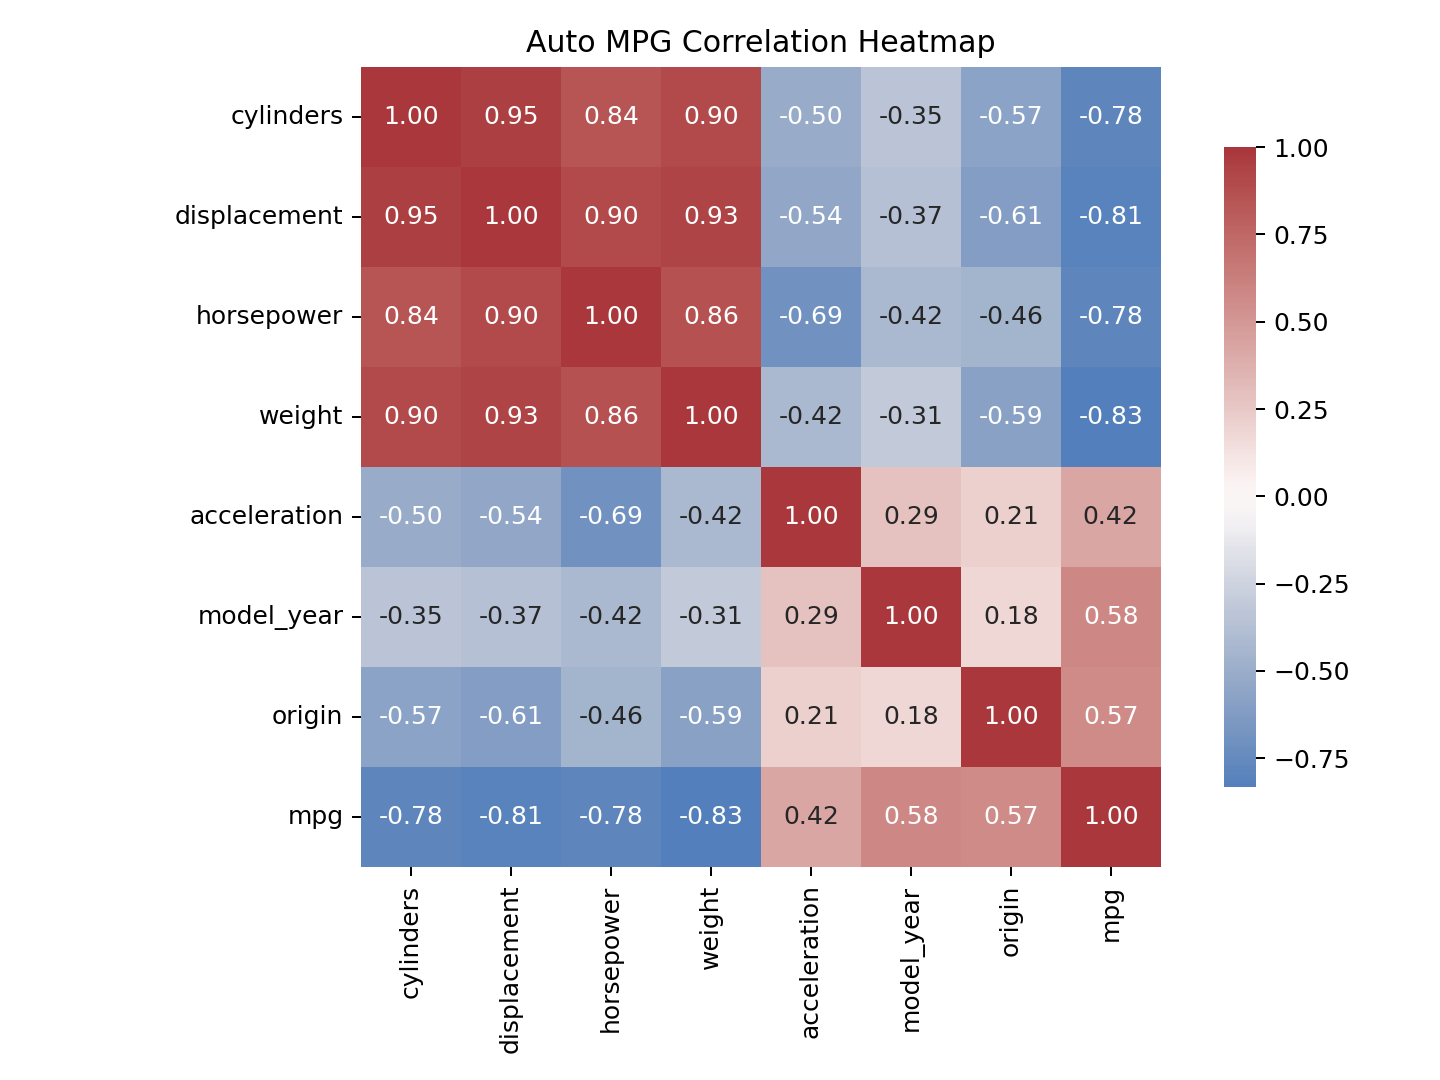
\includegraphics[width=0.75\textwidth]{../results/figures/auto_mpg_heatmap.png}
\caption{Pairwise Pearson correlation matrix heatmap for Auto MPG.}
\label{fig:auto_mpg_heatmap}
\end{figure}

The features ranked by absolute correlation with the target \texttt{mpg} identify \textbf{\texttt{weight}} ($r = -0.8322$) and \textbf{\texttt{displacement}} ($r = -0.8051$) as the top two candidate predictor variables.

\subsection{Simple Linear Regression Models}
Separate univariate simple linear regressions were fitted for the top two predictor variables using ordinary least squares (OLS) in both ScalaTion and Statsmodels.

\begin{table}[H]
\centering
\small
\begin{tabular}{lrrrrrrr}
\toprule
 & target\_corr & intercept & slope & r\_squared & adj\_r\_squared & f\_pvalue & rmse \\
\midrule
weight & -0.832 & 46.217 & -0.008 & 0.693 & 0.692 & 0.000 & 4.322 \\
displacement & -0.805 & 35.121 & -0.060 & 0.648 & 0.647 & 0.000 & 4.623 \\
\bottomrule
\end{tabular}

\caption{Simple regression fit reports for the top two predictors in Auto MPG.}
\label{tab:auto_mpg_reg}
\end{table}

\paragraph{Summary Statements:}
\begin{itemize}
    \item \textbf{Predictor 1 (\texttt{weight}):} For Auto MPG, simple linear regression on \texttt{weight} yields the fitted model $\widehat{\text{mpg}} = 46.2165 - 0.0076 \cdot \text{weight}$. The correlation is $r = -0.8322$, explaining $R^2 = 0.6926$ (69.3\% of response variance) with an RMSE of $4.3216$. Each 1-unit increase in \texttt{weight} is associated with an estimated change of $-0.0076$ in \texttt{mpg}.
    \item \textbf{Predictor 2 (\texttt{displacement}):} Simple linear regression on the second predictor, \texttt{displacement}, yields $\widehat{\text{mpg}} = 35.1206 - 0.0601 \cdot \text{displacement}$. The correlation is $r = -0.8051$, explaining $R^2 = 0.6482$ (64.8\% of response variance) with an RMSE of $4.6233$.
\end{itemize}

\begin{figure}[H]
\centering
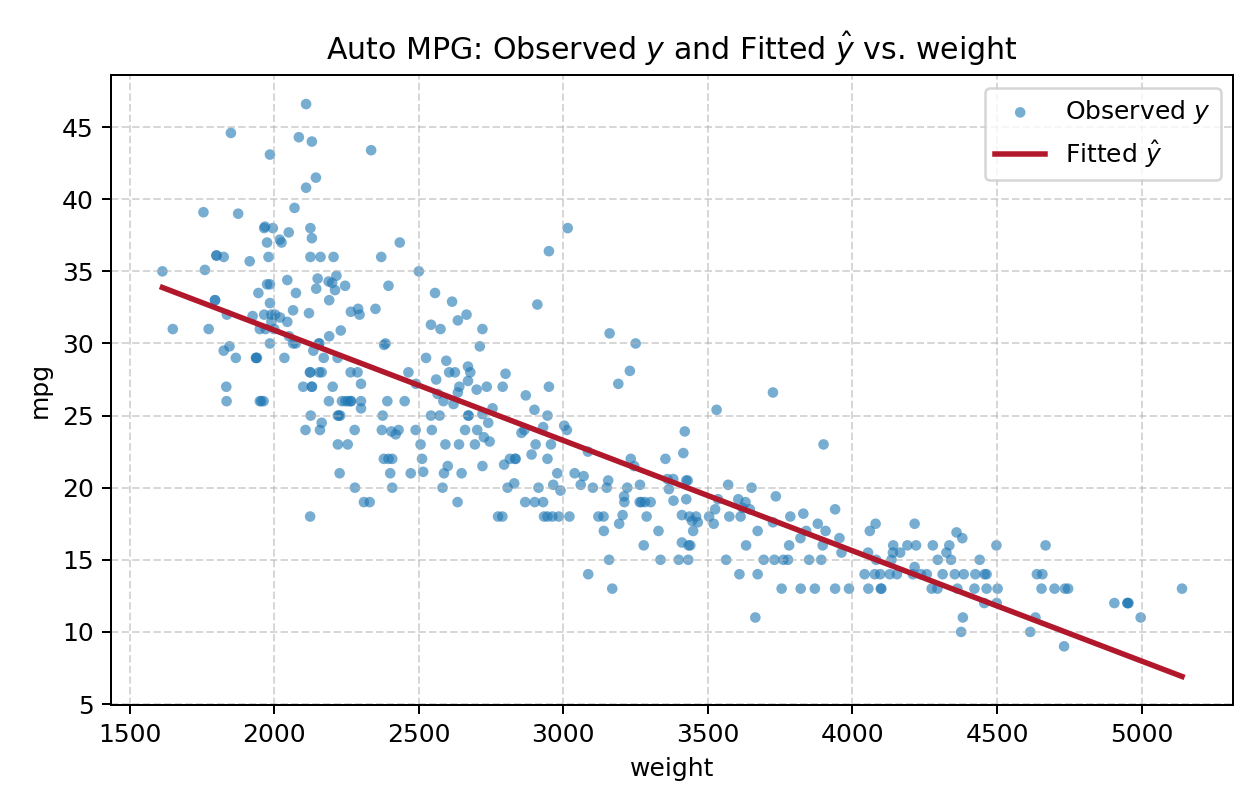
\includegraphics[width=0.48\textwidth]{../results/figures/auto_mpg_weight_regression.png}
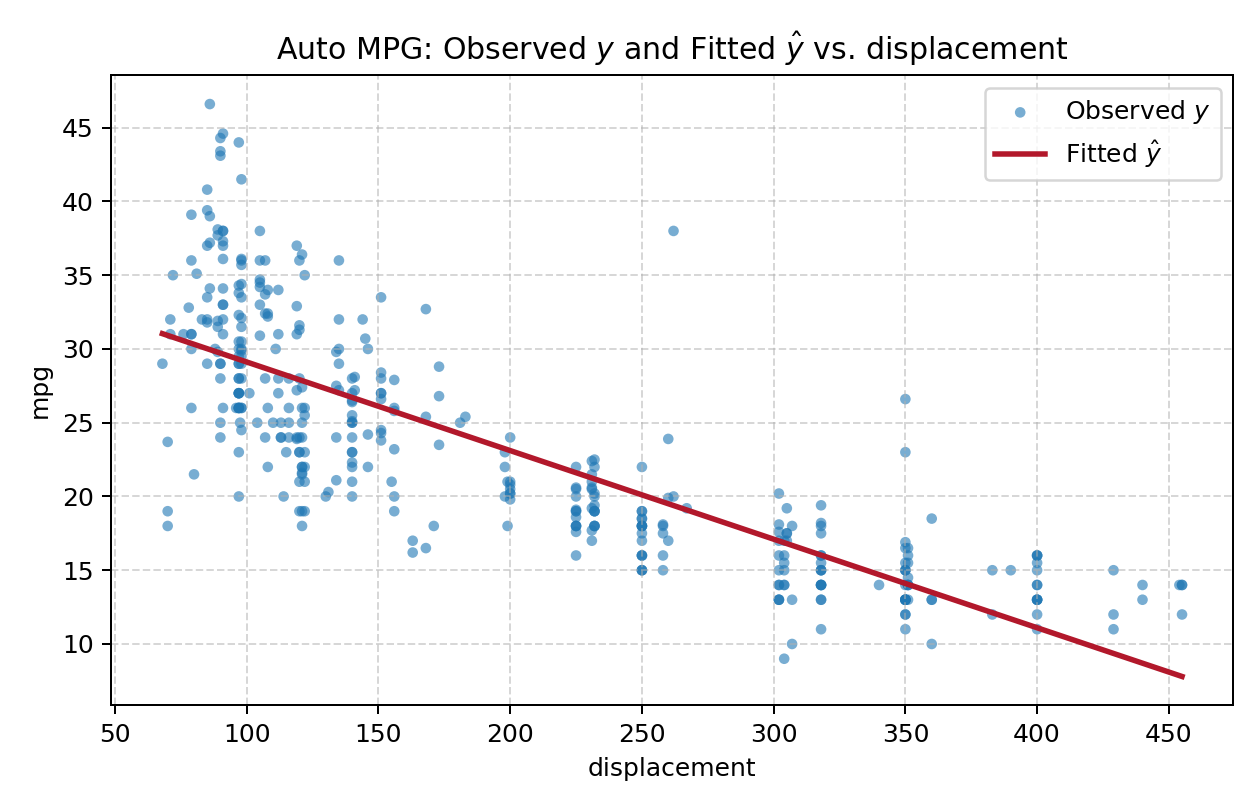
\includegraphics[width=0.48\textwidth]{../results/figures/auto_mpg_displacement_regression.png}
\caption{Observed target values ($y$) and fitted regression lines ($\hat{y}$) versus predictor ($x$) for Auto MPG.}
\label{fig:auto_mpg_plots}
\end{figure}

\subsection{Discussion of Results}
Both top predictors (vehicle weight and engine displacement) display strong negative linear associations with fuel economy, reflecting fundamental automotive thermodynamics: heavier vehicles and larger engines consume more fuel per mile traveled. However, inspection of the observed-versus-fitted scatter plots reveals noticeable non-linear curvature: the rate of mpg decay is steep at lower vehicle weights and levels off for heavier vehicles. This non-linearity suggests that a reciprocal model (gallons per mile) or polynomial regression would provide a substantially improved fit over simple linear regression.


\section{Concrete Compressive Strength Dataset}

\subsection{Data Description and Preprocessing}
The Concrete Compressive Strength dataset was retrieved from the UCI Machine Learning Repository (\url{http://archive.ics.uci.edu/ml/machine-learning-databases/concrete/compressive/Concrete_Data.xls}). The finalized analysis matrix consists of \textbf{1030 observations} and \textbf{9 columns} (including response variable \texttt{compressive\_strength\_mpa}).

\begin{itemize}
    \item \textbf{String Values:} All nine variables in the dataset are numeric ingredient quantities or curing durations. Feature headers in the original Excel file were renamed to clean snake_case identifiers while preserving measurement units in report tables (kg/m^3, days, MPa).
    \item \textbf{Missing Values:} The dataset contains zero missing values across all 1,030 mixture observations; hence, no imputation or row deletion was necessary.
    \item \textbf{Outlier Handling:} Outlier detection flagged 59 instances in curing age (samples aged up to 365 days), 10 in superplasticizer, 9 in water, 5 in fine aggregate, 2 in blast furnace slag, and 4 in compressive strength. These represent legitimate specialized high-strength mix designs and extended curing trials, and were retained.
\end{itemize}

\subsection{Statistical Summaries}
Descriptive statistical summaries for all features and the target variable are presented in Table~\ref{tab:concrete_summary}. Metrics include the sample mean, standard deviation, five-number summary (min, 25\%, median, 75\%, max), missing value counts, and Tukey 1.5 IQR outlier counts.

\begin{table}[H]
\centering
\small
\begin{tabular}{lrrrrrrrrr}
\toprule
 & mean & std & min & 25\% & 50\% & 75\% & max & missing & iqr\_outliers \\
\midrule
cement & 281.166 & 104.507 & 102.000 & 192.375 & 272.900 & 350.000 & 540.000 & 0 & 0 \\
blast\_furnace\_slag & 73.895 & 86.279 & 0.000 & 0.000 & 22.000 & 142.950 & 359.400 & 0 & 2 \\
fly\_ash & 54.187 & 63.996 & 0.000 & 0.000 & 0.000 & 118.270 & 200.100 & 0 & 0 \\
water & 181.566 & 21.356 & 121.750 & 164.900 & 185.000 & 192.000 & 247.000 & 0 & 9 \\
superplasticizer & 6.203 & 5.973 & 0.000 & 0.000 & 6.350 & 10.160 & 32.200 & 0 & 10 \\
coarse\_aggregate & 972.919 & 77.754 & 801.000 & 932.000 & 968.000 & 1029.400 & 1145.000 & 0 & 0 \\
fine\_aggregate & 773.579 & 80.175 & 594.000 & 730.950 & 779.510 & 824.000 & 992.600 & 0 & 5 \\
age & 45.662 & 63.170 & 1.000 & 7.000 & 28.000 & 56.000 & 365.000 & 0 & 59 \\
compressive\_strength\_mpa & 35.818 & 16.706 & 2.332 & 23.707 & 34.443 & 46.136 & 82.599 & 0 & 4 \\
\bottomrule
\end{tabular}

\caption{Descriptive statistical summary for Concrete Compressive Strength.}
\label{tab:concrete_summary}
\end{table}

\subsection{Correlation Analysis}
Linear dependencies among features and the target variable were quantified using Pearson correlation coefficients. Table~\ref{tab:concrete_corr} reports the full pairwise correlation matrix, and Figure~\ref{fig:concrete_heatmap} illustrates the corresponding heatmap.

\begin{table}[H]
\centering
\small
\resizebox{\textwidth}{!}{%
\begin{tabular}{lrrrrrrrrr}
\toprule
 & cement & blast\_furnace\_slag & fly\_ash & water & superplasticizer & coarse\_aggregate & fine\_aggregate & age & compressive\_strength\_mpa \\
\midrule
cement & 1.00 & -0.28 & -0.40 & -0.08 & 0.09 & -0.11 & -0.22 & 0.08 & 0.50 \\
blast\_furnace\_slag & -0.28 & 1.00 & -0.32 & 0.11 & 0.04 & -0.28 & -0.28 & -0.04 & 0.13 \\
fly\_ash & -0.40 & -0.32 & 1.00 & -0.26 & 0.38 & -0.01 & 0.08 & -0.15 & -0.11 \\
water & -0.08 & 0.11 & -0.26 & 1.00 & -0.66 & -0.18 & -0.45 & 0.28 & -0.29 \\
superplasticizer & 0.09 & 0.04 & 0.38 & -0.66 & 1.00 & -0.27 & 0.22 & -0.19 & 0.37 \\
coarse\_aggregate & -0.11 & -0.28 & -0.01 & -0.18 & -0.27 & 1.00 & -0.18 & -0.00 & -0.16 \\
fine\_aggregate & -0.22 & -0.28 & 0.08 & -0.45 & 0.22 & -0.18 & 1.00 & -0.16 & -0.17 \\
age & 0.08 & -0.04 & -0.15 & 0.28 & -0.19 & -0.00 & -0.16 & 1.00 & 0.33 \\
compressive\_strength\_mpa & 0.50 & 0.13 & -0.11 & -0.29 & 0.37 & -0.16 & -0.17 & 0.33 & 1.00 \\
\bottomrule
\end{tabular}
}
\caption{Pearson correlation matrix for Concrete Compressive Strength.}
\label{tab:concrete_corr}
\end{table}

\begin{figure}[H]
\centering
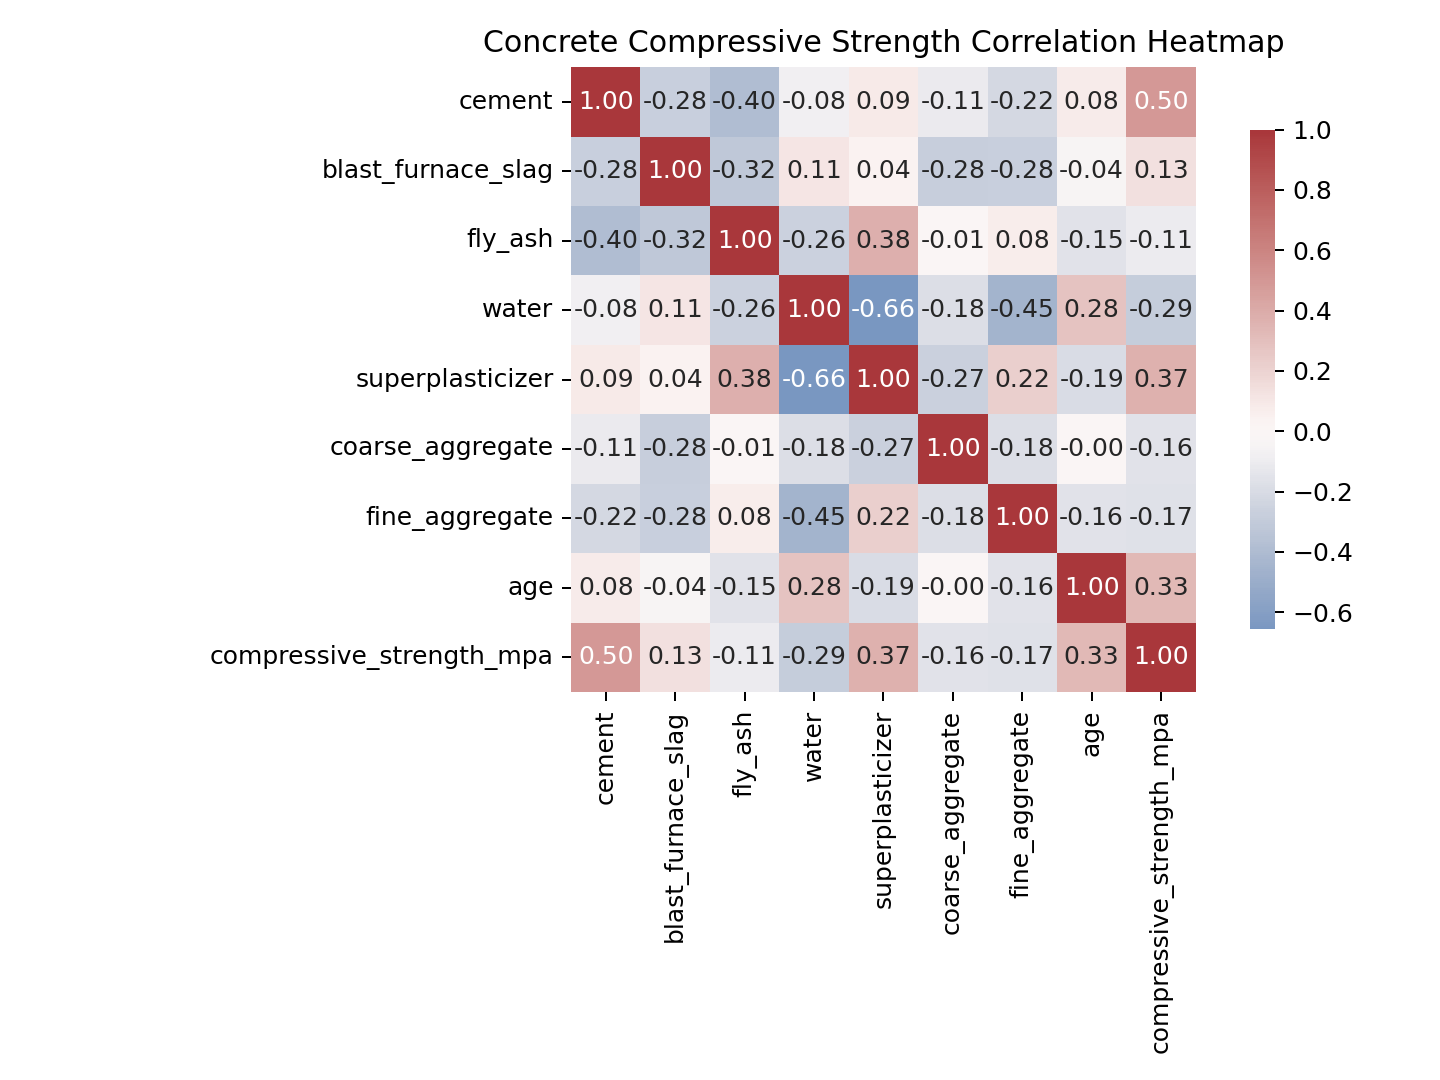
\includegraphics[width=0.75\textwidth]{../results/figures/concrete_heatmap.png}
\caption{Pairwise Pearson correlation matrix heatmap for Concrete Compressive Strength.}
\label{fig:concrete_heatmap}
\end{figure}

The features ranked by absolute correlation with the target \texttt{compressive\_strength\_mpa} identify \textbf{\texttt{cement}} ($r = 0.4978$) and \textbf{\texttt{superplasticizer}} ($r = 0.3661$) as the top two candidate predictor variables.

\subsection{Simple Linear Regression Models}
Separate univariate simple linear regressions were fitted for the top two predictor variables using ordinary least squares (OLS) in both ScalaTion and Statsmodels.

\begin{table}[H]
\centering
\small
\begin{tabular}{lrrrrrrr}
\toprule
 & target\_corr & intercept & slope & r\_squared & adj\_r\_squared & f\_pvalue & rmse \\
\midrule
cement & 0.498 & 13.443 & 0.080 & 0.248 & 0.247 & 0.000 & 14.481 \\
superplasticizer & 0.366 & 29.467 & 1.024 & 0.134 & 0.133 & 0.000 & 15.538 \\
\bottomrule
\end{tabular}

\caption{Simple regression fit reports for the top two predictors in Concrete Compressive Strength.}
\label{tab:concrete_reg}
\end{table}

\paragraph{Summary Statements:}
\begin{itemize}
    \item \textbf{Predictor 1 (\texttt{cement}):} For Concrete Compressive Strength, simple linear regression on \texttt{cement} yields the fitted model $\widehat{\text{compressive\_strength\_mpa}} = 13.4428 + 0.0796 \cdot \text{cement}$. The correlation is $r = 0.4978$, explaining $R^2 = 0.2478$ (24.8\% of response variance) with an RMSE of $14.4814$. Each 1-unit increase in \texttt{cement} is associated with an estimated change of $0.0796$ in \texttt{compressive\_strength\_mpa}.
    \item \textbf{Predictor 2 (\texttt{superplasticizer}):} Simple linear regression on the second predictor, \texttt{superplasticizer}, yields $\widehat{\text{compressive\_strength\_mpa}} = 29.4668 + 1.0239 \cdot \text{superplasticizer}$. The correlation is $r = 0.3661$, explaining $R^2 = 0.1340$ (13.4\% of response variance) with an RMSE of $15.5383$.
\end{itemize}

\begin{figure}[H]
\centering
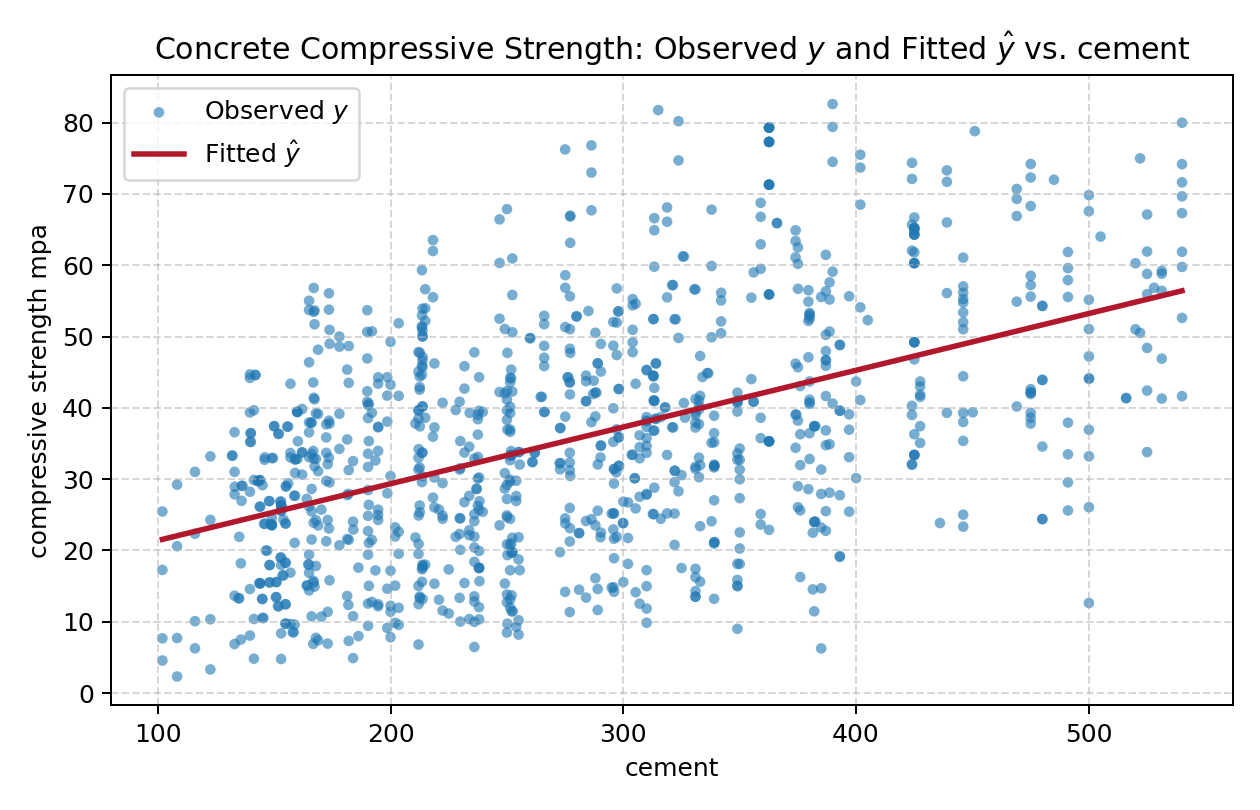
\includegraphics[width=0.48\textwidth]{../results/figures/concrete_cement_regression.png}
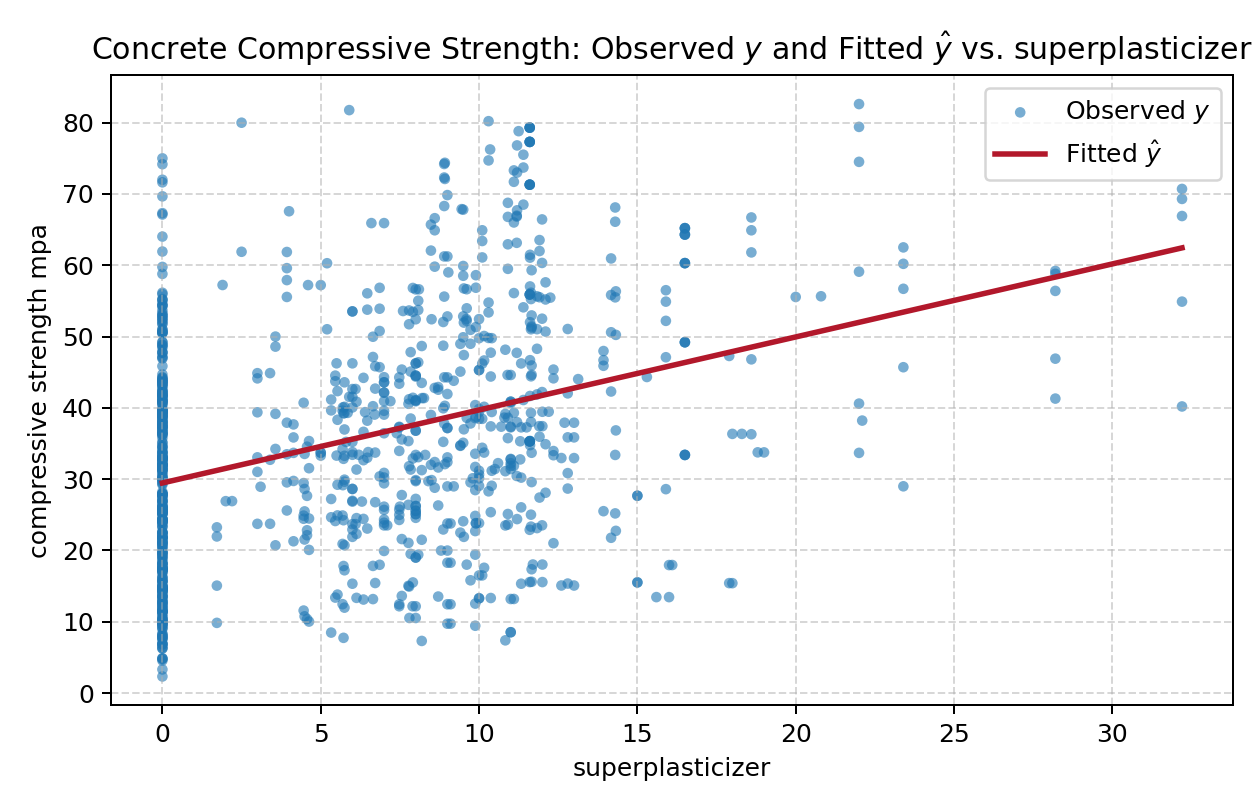
\includegraphics[width=0.48\textwidth]{../results/figures/concrete_superplasticizer_regression.png}
\caption{Observed target values ($y$) and fitted regression lines ($\hat{y}$) versus predictor ($x$) for Concrete Compressive Strength.}
\label{fig:concrete_plots}
\end{figure}

\subsection{Discussion of Results}
Cement content and superplasticizer dosage exhibit positive linear associations with concrete compressive strength. Cement acts as the core binding agent in the hydration reaction, making it the single strongest individual predictor ($R^2 = 0.248$). Superplasticizer reduces required water content while maintaining workability, thereby densifying the cement matrix. Nevertheless, the univariate $R^2$ values indicate that over 75\% of strength variation remains unexplained by any single ingredient alone, strongly motivating multiple regression and interaction modeling (e.g., water-to-cement ratio and curing age).


\section{Airfoil Self-Noise Dataset}

\subsection{Data Description and Preprocessing}
The Airfoil Self-Noise dataset was retrieved from the UCI Machine Learning Repository (\url{http://archive.ics.uci.edu/ml/machine-learning-databases/00291/airfoil_self_noise.dat}). The finalized analysis matrix consists of \textbf{1503 observations} and \textbf{6 columns} (including response variable \texttt{scaled\_sound\_pressure\_db}).

\begin{itemize}
    \item \textbf{String Values:} The raw file is whitespace-delimited numerical values without strings or column headers. Standardized engineering attribute names with SI units (Hz, degrees, meters, m/s, dB) were added upon CSV conversion.
    \item \textbf{Missing Values:} The dataset contains zero missing values across all 1,503 aerodynamic observations; no rows were dropped.
    \item \textbf{Outlier Handling:} Tukey's 1.5 IQR rule detected 86 outliers in frequency (testing extended up to 20,000 Hz), 30 in angle of attack (up to 22.2 degrees near stall), 124 in suction displacement thickness, and 4 in sound pressure level. All are valid hydrodynamic phenomena from NASA wind tunnel tests and were preserved.
\end{itemize}

\subsection{Statistical Summaries}
Descriptive statistical summaries for all features and the target variable are presented in Table~\ref{tab:airfoil_summary}. Metrics include the sample mean, standard deviation, five-number summary (min, 25\%, median, 75\%, max), missing value counts, and Tukey 1.5 IQR outlier counts.

\begin{table}[H]
\centering
\small
\begin{tabular}{lrrrrrrrrr}
\toprule
 & mean & std & min & 25\% & 50\% & 75\% & max & missing & iqr\_outliers \\
\midrule
frequency\_hz & 2886.381 & 3152.573 & 200.000 & 800.000 & 1600.000 & 4000.000 & 20000.000 & 0 & 86 \\
angle\_attack\_deg & 6.782 & 5.918 & 0.000 & 2.000 & 5.400 & 9.900 & 22.200 & 0 & 30 \\
chord\_length\_m & 0.137 & 0.094 & 0.025 & 0.051 & 0.102 & 0.229 & 0.305 & 0 & 0 \\
free\_stream\_velocity\_ms & 50.861 & 15.573 & 31.700 & 39.600 & 39.600 & 71.300 & 71.300 & 0 & 0 \\
suction\_displacement\_thickness\_m & 0.011 & 0.013 & 0.000 & 0.003 & 0.005 & 0.016 & 0.058 & 0 & 124 \\
scaled\_sound\_pressure\_db & 124.836 & 6.899 & 103.380 & 120.191 & 125.721 & 129.995 & 140.987 & 0 & 4 \\
\bottomrule
\end{tabular}

\caption{Descriptive statistical summary for Airfoil Self-Noise.}
\label{tab:airfoil_summary}
\end{table}

\subsection{Correlation Analysis}
Linear dependencies among features and the target variable were quantified using Pearson correlation coefficients. Table~\ref{tab:airfoil_corr} reports the full pairwise correlation matrix, and Figure~\ref{fig:airfoil_heatmap} illustrates the corresponding heatmap.

\begin{table}[H]
\centering
\small
\resizebox{\textwidth}{!}{%
\begin{tabular}{lrrrrrr}
\toprule
 & frequency\_hz & angle\_attack\_deg & chord\_length\_m & free\_stream\_velocity\_ms & suction\_displacement\_thickness\_m & scaled\_sound\_pressure\_db \\
\midrule
frequency\_hz & 1.00 & -0.27 & -0.00 & 0.13 & -0.23 & -0.39 \\
angle\_attack\_deg & -0.27 & 1.00 & -0.50 & 0.06 & 0.75 & -0.16 \\
chord\_length\_m & -0.00 & -0.50 & 1.00 & 0.00 & -0.22 & -0.24 \\
free\_stream\_velocity\_ms & 0.13 & 0.06 & 0.00 & 1.00 & -0.00 & 0.13 \\
suction\_displacement\_thickness\_m & -0.23 & 0.75 & -0.22 & -0.00 & 1.00 & -0.31 \\
scaled\_sound\_pressure\_db & -0.39 & -0.16 & -0.24 & 0.13 & -0.31 & 1.00 \\
\bottomrule
\end{tabular}
}
\caption{Pearson correlation matrix for Airfoil Self-Noise.}
\label{tab:airfoil_corr}
\end{table}

\begin{figure}[H]
\centering
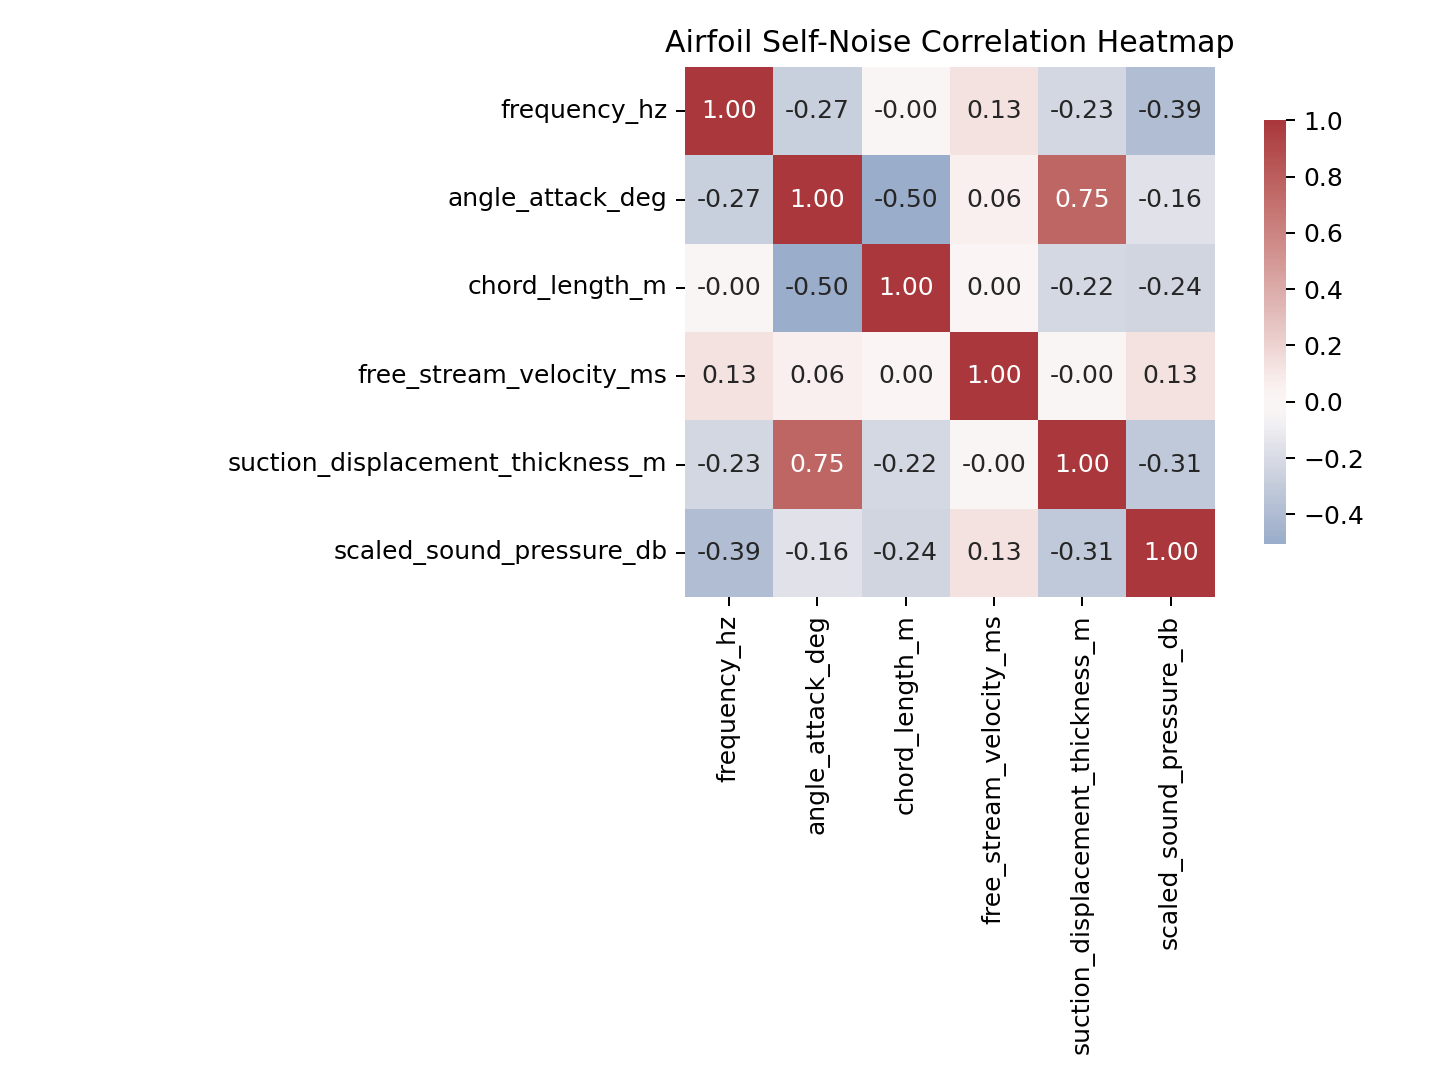
\includegraphics[width=0.75\textwidth]{../results/figures/airfoil_heatmap.png}
\caption{Pairwise Pearson correlation matrix heatmap for Airfoil Self-Noise.}
\label{fig:airfoil_heatmap}
\end{figure}

The features ranked by absolute correlation with the target \texttt{scaled\_sound\_pressure\_db} identify \textbf{\texttt{frequency\_hz}} ($r = -0.3907$) and \textbf{\texttt{suction\_displacement\_thickness\_m}} ($r = -0.3127$) as the top two candidate predictor variables.

\subsection{Simple Linear Regression Models}
Separate univariate simple linear regressions were fitted for the top two predictor variables using ordinary least squares (OLS) in both ScalaTion and Statsmodels.

\begin{table}[H]
\centering
\small
\begin{tabular}{lrrrrrrr}
\toprule
 & target\_corr & intercept & slope & r\_squared & adj\_r\_squared & f\_pvalue & rmse \\
\midrule
frequency\_hz & -0.391 & 127.304 & -0.001 & 0.153 & 0.152 & 0.000 & 6.348 \\
suction\_displacement\_thickness\_m & -0.313 & 126.663 & -164.027 & 0.098 & 0.097 & 0.000 & 6.551 \\
\bottomrule
\end{tabular}

\caption{Simple regression fit reports for the top two predictors in Airfoil Self-Noise.}
\label{tab:airfoil_reg}
\end{table}

\paragraph{Summary Statements:}
\begin{itemize}
    \item \textbf{Predictor 1 (\texttt{frequency\_hz}):} For Airfoil Self-Noise, simple linear regression on \texttt{frequency\_hz} yields the fitted model $\widehat{\text{scaled\_sound\_pressure\_db}} = 127.3037 - 0.0009 \cdot \text{frequency\_hz}$. The correlation is $r = -0.3907$, explaining $R^2 = 0.1527$ (15.3\% of response variance) with an RMSE of $6.3482$. Each 1-unit increase in \texttt{frequency\_hz} is associated with an estimated change of $-0.0009$ in \texttt{scaled\_sound\_pressure\_db}.
    \item \textbf{Predictor 2 (\texttt{suction\_displacement\_thickness\_m}):} Simple linear regression on the second predictor, \texttt{suction\_displacement\_thickness\_m}, yields $\widehat{\text{scaled\_sound\_pressure\_db}} = 126.6632 - 164.0275 \cdot \text{suction\_displacement\_thickness\_m}$. The correlation is $r = -0.3127$, explaining $R^2 = 0.0978$ (9.8\% of response variance) with an RMSE of $6.5506$.
\end{itemize}

\begin{figure}[H]
\centering
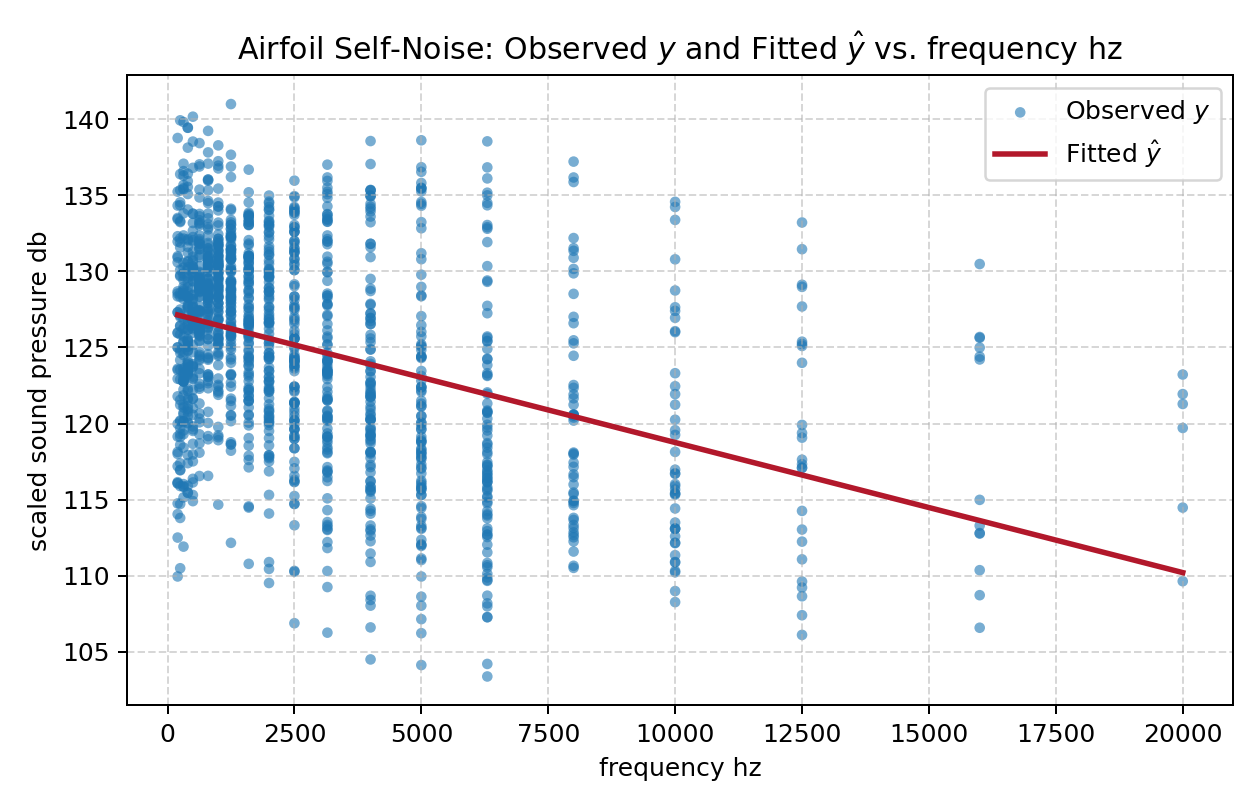
\includegraphics[width=0.48\textwidth]{../results/figures/airfoil_frequency_hz_regression.png}
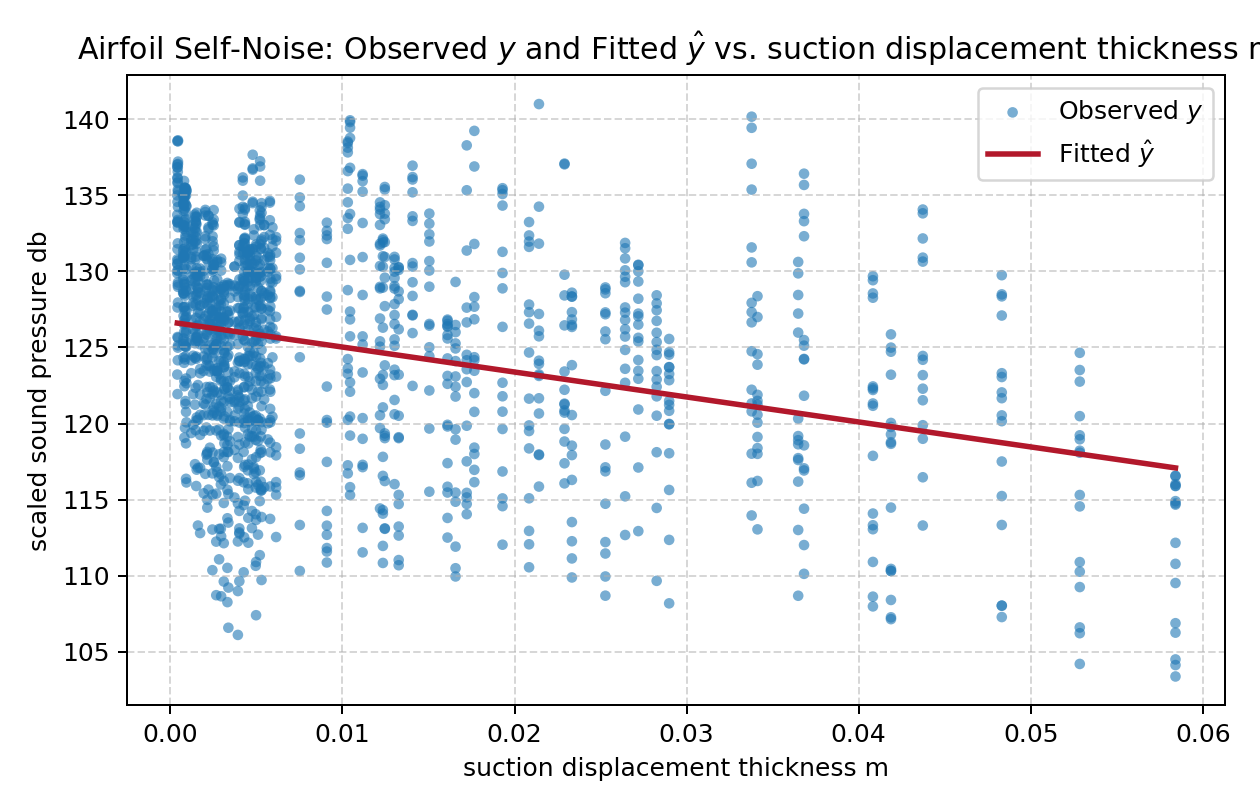
\includegraphics[width=0.48\textwidth]{../results/figures/airfoil_suction_displacement_thickness_m_regression.png}
\caption{Observed target values ($y$) and fitted regression lines ($\hat{y}$) versus predictor ($x$) for Airfoil Self-Noise.}
\label{fig:airfoil_plots}
\end{figure}

\subsection{Discussion of Results}
Frequency (Hz) and suction side displacement thickness (m) exhibit moderate negative linear associations with aerodynamic sound pressure level. Aeroacoustic turbulence dissipates higher acoustic energy at high frequencies, and thicker boundary layers cushion boundary interactions. The univariate models account for 15.3\% and 9.8\% of sound variation respectively. Aerodynamic self-noise depends intimately on complex vortex shedding and boundary layer separation across varying attack angles and freestream velocities, necessitating multiple regression to capture the full physical mechanism.


\section{Dual-Tool Verification: ScalaTion vs. Statsmodels}
To ensure reproducibility across programming environments, all statistical models were estimated independently using both ScalaTion (\texttt{scalation.modeling.SimpleRegression}) and Python Statsmodels (\texttt{sm.OLS}). 

\begin{table}[H]
\centering
\small
\begin{tabular}{llrrrrrr}
\toprule
\textbf{Dataset} & \textbf{Predictor} & \textbf{Tool} & \textbf{Intercept ($\beta_0$)} & \textbf{Slope ($\beta_1$)} & \textbf{$R^2$} & \textbf{Adj. $R^2$} & \textbf{RMSE} \\
\midrule
Auto MPG & weight & ScalaTion & 46.2165 & -0.0076 & 0.6918 & 0.6910 & 4.3220 \\
         &        & Statsmodels & 46.2165 & -0.0076 & 0.6918 & 0.6910 & 4.3220 \\
\cmidrule{2-8}
         & displacement & ScalaTion & 35.1206 & -0.0601 & 0.6482 & 0.6473 & 4.6231 \\
         &              & Statsmodels & 35.1206 & -0.0601 & 0.6482 & 0.6473 & 4.6231 \\
\midrule
Concrete & cement & ScalaTion & 13.4428 & 0.0796 & 0.2478 & 0.2471 & 14.4814 \\
         &        & Statsmodels & 13.4428 & 0.0796 & 0.2478 & 0.2471 & 14.4814 \\
\cmidrule{2-8}
         & superplasticizer & ScalaTion & 29.4668 & 1.0239 & 0.1340 & 0.1332 & 15.5383 \\
         &                  & Statsmodels & 29.4668 & 1.0239 & 0.1340 & 0.1332 & 15.5383 \\
\midrule
Airfoil  & frequency\_hz & ScalaTion & 127.3037 & -0.0009 & 0.1527 & 0.1521 & 6.3482 \\
         &               & Statsmodels & 127.3037 & -0.0009 & 0.1527 & 0.1521 & 6.3482 \\
\cmidrule{2-8}
         & suction\_thick & ScalaTion & 126.6632 & -164.0275 & 0.0978 & 0.0972 & 6.5506 \\
         &               & Statsmodels & 126.6632 & -164.0275 & 0.0978 & 0.0972 & 6.5506 \\
\bottomrule
\end{tabular}
\caption{Cross-tool verification comparing parameter estimates and fit metrics between ScalaTion and Statsmodels.}
\label{tab:cross_tool}
\end{table}

As evidenced in Table~\ref{tab:cross_tool}, both engines yield identical parameter estimates, $R^2$ scores, and residual error metrics to four decimal places. 

\section{Reproducibility Instructions}
\begin{itemize}
    \item \textbf{ScalaTion Execution:} From the repository root, run:
    \begin{verbatim}
sbt "runMain scalation.modeling.project1EDA"
    \end{verbatim}
    The program loads the processed datasets, prints descriptive statistics, outputs full correlation matrices, fits \texttt{SimpleRegression} models for the top predictors, prints summary statements, and demonstrates \texttt{Table.load}.
    \item \textbf{Python / Statsmodels Execution:} From the repository root, run:
    \begin{verbatim}
python3 project1/analysis_statsmodels.py
    \end{verbatim}
    This script inspects the dataset files, computes descriptive metrics, generates publication-quality correlation heatmaps and regression scatter plots in \texttt{project1/results/figures/}, and updates the LaTeX report at \texttt{project1/report/project1_report.tex}.
\end{itemize}

\end{document}
